\documentclass[a4j,12pt]{jarticle}
\usepackage[dvipdfmx]{graphicx}
\usepackage[dvipdfmx]{hyperref}
%
% ---- 本文中でプログラムを掲載する際にキャプションを「リスト1」のようにする設定
%
% http://en.wikibooks.org/wiki/LaTeX/Floats,_Figures_and_Captions#Custom_floats
% 本文中でリストと表現されているところは
%
% \begin{program}..\end{program}を使います。
%
%  \begin{program}\centering
%  \begin{verbatim}
%
%  #define COM1_PORT (0x3f8)
%  #define COM1_LSR (COM1_PORT + 0)
%  #define COM1_RBR (COM1_PORT + 5)
%  unsigned char read_reg_byte(unsigned short port) {
%    unsigned char val;
%    asm volatile("inb %1, %0" : "=a"(val) : "Nd"(port));
%    return val;
%  }
%  \end{verbatim}
%  \caption{I/O マップド I/O での read\_reg\_byte() 関数およびレジスタの宣言}
%  \end{program}
%
% TODO: programをリストに変更する
%
\usepackage{float}
% 例では次のようになっているが...
%\newfloat{program}{thp}{lop}
\newfloat{program}{thp}{lop}
% ------------------------------------------------------------------------------

\title{第 6 回 Intel VT-xを用いたハイパーバイザの実装「仮想CPUの実行処理・その1」}
\author{Takuya ASADA syuu@dokukino.com}

\begin{document}

\maketitle

\section{はじめに}

 前回までに、5回にわたりハードウェアが提供して
いる仮想化支援機能を解説しました。
 今回からは、実際にどのようにして仮想化支援機
構を使い、ハイパーバイザを実装するのかを解説し
ていきます。解説には、実装の具体例として現在
FreeBSDへの実装が進められているハイパーバイザ
「BHyVe (ビーハイブ)」を用います。


\section{BHyVeとは}

 BHyVeはNetAppにより開発された、FreeBSDで
動く新しいハイパーバイザです。 2011年に発表され、
実装が進められています。現在、FreeBSD10の新機
能の1つとしてリリースすることを目指しています
\footnote{2013年1月にFreeBSD-CURRENTの開発ツリーにマージされました。}。
設計はLinux KVMに似ており、FreeBSD版の
KVMとも言えるでしょう。ただし、BHyVeは現在開
発の初期段階であるため、現在のKVMに比べ非常
に機能は限られています。現状、実用に用いるのは
難しい開発版の機能となります。しかし、ハイパー
バイザの実装方法を学ぶための教材としては、以下
の二点が優れています。
 1つは、最低限の機能のみ実装しているためKVM
と比べるとコード量が非常にコンパクトであること
です。もう1つは、デバイスエミュレーションなど
を行うユーザランドプログラム(詳細は後述)がシン
プルなものであることです。KVMではユーザランド
プログラムに既存のエミュレータであるQEMUを流
用しており、これにより既存OSとの高い互換性が
得られていますがコードの見通しが悪くなっていま
す。そこで、本連載ではKVMではなくBHyVeを用
いて解説を行うことにします。

\section{解説対象のバージョン}

 BHyVeは現在、リリース版が存在しません。ま
た、開発の初期段階であるため、大きな変更が加え
られることも予想されます。
  そこで、本連載では現時点でのFreeBSD-
CURRENTでスナップショットが公開されている最
新リビジョンであるr245673を用いて解説を行いま
す。 r245673のインストールディスクは、次のアドレ
スからダウンロードできます。

\url{ftp://ftp.freebsd.org/pub/FreeBSD/snapshots/amd64/amd64/ISO-IMAGES/10.0/FreeBSD-10.0-CURRENT-amd64-20130119-r245673-release.iso}

 r245673のソースコードは次のコマンドで取得で
きます。

svn co -r245673 svn://svn.freebsd.org/base/head src

 また、BHyVe用にコンフィグレーションされたゲ
ストマシンのディスクイメージが配布さ れており、
次のアドレスからダウンロードできます。

\url{http://mirrors.nycbug.org/pub/BHyVe/r244024/diskdev.xz}


\section{BHyVeの動作環境}

 BHyVeを試すには、Intel VT-xとEPT(Extended
Page Tables)をサポートしたCPUが 必要です。
 今のところAMDのCPUには対応していません。
どのモデルのCPUがEPTをサポートしているかは
ark.intel.comで調べられます。簡単な目安としては、
Core i3, i5, i7ならばほぼすべてのCPUが対応して
います。CeleronやPentiumなどの廉価版CPUでも
EPT対応モデルが一部存在しています。実機にイン
ストールするのが最も確実ですが、最近のVMware
(VMware Player・VMware Workstation・VMware
Fusion)ならばNested VM
\footnote{ハイパーバイザ上でハイパーバイザを実行可能にする機能。}
に対応しているため仮想マシン上で試すこともできます。

\section{BHyVeが提供する機能}

 現状、BHyVeではゲストOSとしてFreeBSD/
amd64だけをサポートしています。
 ハードディスクコントローラとしては、標準的な
IDEやAHCIコントローラのエミュレーションはサ
ポートせず、準仮想化ドライバであるvirtio-blkをサ
ポートしています。
 NICコントローラとしても同様に、標準的なIntel
e1000などのデバイスのエミュレーションをサポー
トせず、準仮想化ドライバであるvirtio-netをサポー
トしています。virtioは多くの場合、標準的なデバイ
スのエミュレーションと比較して高い性能が得られ
ますが、ゲストOSにvirtioドライバをインストール
し、/boot/loader.confの設定を行う必要があります。
システムコンソールとしては、標準的なビデオデバ
イスをサポートはサポートされず、PCI接続の16550
互換シリアルポートのみをサポートしています。
PCI接続のシリアルポートをシステムコンソールと
して使うのは非標準的なハードウェア構成であるた
め、これについても/boot/loader.confの設定を行う
必要があります。また、ビデオデバイスをサポート
しないため、X11を起動してGUI環境を表示するこ
とはできません。
 BHyVeがエミュレート可能なデバイスは上述の3
種類だけですが、Intel VT-dを用いて実機上のPCI・
PCI Expressデバイスをゲストマシンへパススルー
接続できます。この他、割り込みコントローラのエ
ミュレーション(Local APIC、IO-APIC)や、タイマ
デバイスのエミュレーション、ハードウェア構成を
ゲストOSへ伝えるのに必要なAPICなどをサポー
トしています。また、BIOSやUEFIなどのファーム
ウェアをサポートしていないため、ディスクイメー
ジからブートローダをロードしてゲストOSを起動
することができません。このためにハイパーバイザ
の機能としてFreeBSDカーネルをロードしゲストマ
シンを初期化するOSローダが実装されています。


\section{BHyVeの構成}

 BHyVeは、カーネルモジュールとユーザランドプ
ラグラムの2つから構成されます。
 カーネルモジュールvmm.koは、CPUに対して
VT-x命令を発効するなど、ハードウェアに近い処理
を行います。
 ユーザランドプログラム/usr/sbin/bhyveは、ユー
ザインタフェースを提供し、ハードウェアエミュ
レーションを行います。
 また、BHyVeには/usr/sbin/bhyveloadというツー
ルがあります。前章で述べた通り、BHyVeではディ
スクイメージ上のブートローダを実行できません。
このため、ゲストカーネルをロードして起動可能な
状態に初期化するゲストOSローダ(/usr/sbin/bhyveload)
が付属します。
 /usr/sbin/bhyveloadはFreeBSDブートローダを
FreeBSD上で実行可能なプログラムに改変し、ゲ
ストマシンのディスクイメージからカーネルを読み
込んでゲストメモリ空間へ展開するようにしたもの
です。/usr/sbin/bhyveloadを実行すると、FreeBSD
のブート時に表示されるのと同じメニューが表示さ
れます。このため、一見するとゲストマシンの実行
が開始されたように見えます。しかし、これはホス
トOSで/usr/sbin/bhyveloadが出力している画面で、
ゲストマシンの起動は開始されていません。
 このほか、ゲストマシンの実行とは直接関係しま
せんが、VMインスタンスの削除などを行うための
VMインスタンス管理ツールとして/usr/sbin/bhyvectl
が提供されています。
 これらのユーザランドのプログラム群は、VM管理
用のライブラリ(libvmmapi)を通してゲストマシンの
初期化や実行をします。libvmmapiはmmapやioctlを
発行し、vmm.koが提供するデバイスを操作します。
 全体図を図1に示します。

\begin{figure}
 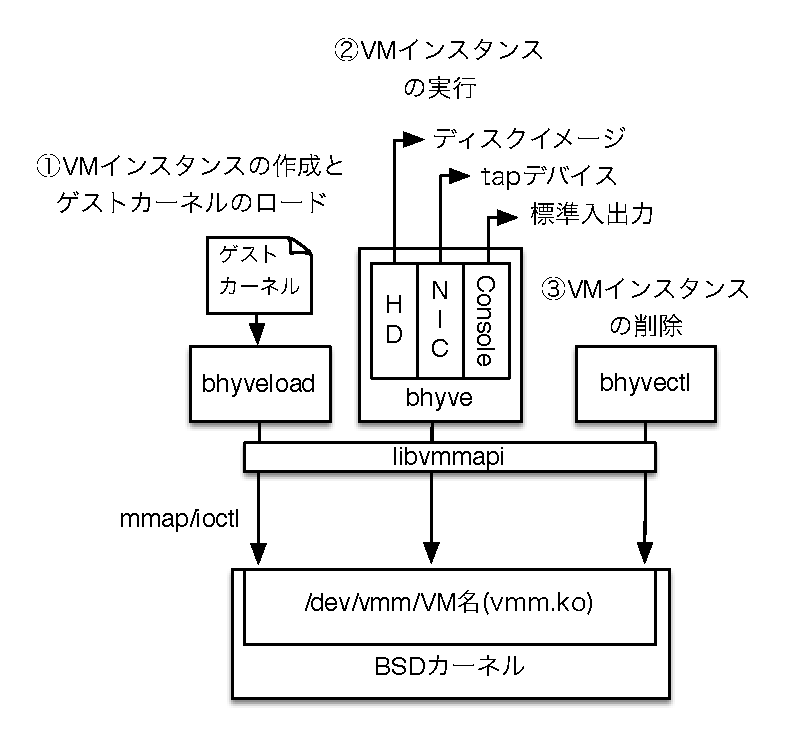
\includegraphics{figures/part6_fig1.eps}
 \caption{BHyVeの構成}
 \label{fig1}
\end{figure}

\section{BHyVeの使い方}

 BHyVeを試すには、ホストマシンのセットアップ
とゲストマシンのディスクイメージの準備が必要で
す。前述のアドレスを参照してください。
 図\ref{fig2}にシェルからBHyVeを用いてゲストマシ
ンを実行する方法を示します。

\begin{figure}\centering
{\tiny
\begin{verbatim}
# kldload vmm.ko <------------------------------|(1)カーネルモジュールをロードし、BHyVeを使用可能にする|
# ls /dev/vmm <----------------------------------------+---------------------------------------------+
# /usr/sbin/bhyveload -d diskdev -m 1024 guest0 <---+  |(2)vmm.koがロードされると/dev/vmmディレクトリ|
                                                    |  |が作成される。この状態ではVMインスタンスが存 |
Consoles: userboot                                  |  |在しないので、ディレクトリは空               |
                                                    |  +---------------------------------------------+
FreeBSD/amd64 User boot, Revision 1.1               +---------------------------------------------+
(root@bhyve, Sat Dec  8 17:35:59 PST 2012)                                                        |
Loading /boot/defaults/loader.conf                                                                |
/boot/kernel/kernel text=0xd01c58 data=0x15e9a0+0x2bb490 syms=[0x8+0x14bbd8+0x8+0x1a7a89]         v
/boot/kernel/virtio.ko size 0x5a90 at 0x1810000        +----------------------------------------------+
/boot/kernel/if_vtnet.ko size 0xd910 at 0x1816000      |(3) /usr/sbin/bhyveloadはVMインスタンスを作成 |
/boot/kernel/virtio_pci.ko size 0x6cc0 at 0x1824000    |し、BSDカーネルをディスクイメージから読み込み |
/boot/kernel/virtio_blk.ko size 0x6b08 at 0x182b000    |ます。そしてVMインスタンスのメモリ領域へロード|
|                                                      |して起動可能な状態を作る。カーネルをロードする|
                                                       |プログラムはFreeBSDのブートローダのコードをそ |
  ______               ____   _____ _____              |のまま使っているため、ブート時に表示されるのと|
 |  ____|             |  _ \ / ____|  __ \             |同じメニューが表示される。しかし、これはホスト|
 | |___ _ __ ___  ___ | |_) | (___ | |  | |            |側で実行されているプログラムでゲストマシンの起|
 |  ___| '__/ _ \/ _ \|  _ < \___ \| |  | |            |動は始まってない。引数-dはディスクイメージ、-m|
 | |   | | |  __/  __/| |_) |____) | |__| |            |はメモリサイズ、最後の引数はVM名を指定している|
 | |   | | |    |    ||     |      |      |            +----------------------------------------------+
 |_|   |_|  \___|\___||____/|_____/|_____/    ```                       `
                                             s` `.....---.......--```   -/
 ?????????????Welcome to FreeBSD???????????? +o   .--`         /y:`     +.
 ?                                         ?  yo`:.            :o     `+-
 ?  1. Boot Multi User [Enter]             ?   y/               -/`  -o/
 ?  2. Boot [S]ingle User                  ?  .-                  ::/sy+:.
 ?  3. [Esc]ape to loader prompt           ?  /                     `--  /
 ?  4. Reboot                              ? `:                          :`
 ?                                         ? `:                          :`
 ?  Options:                               ?  /                          /
 ?  5. Configure Boot [O]ptions...         ?  .-                        -.
 ?                                         ?   --                      -.
 ?                                         ?    `:`                  `:`
 ?                                         ?      .--             `--.
 ?                                         ?         .---.....----.
 ???????????????????????????????????????????
                                                 +---------------------------------------------------+
Booting...                                       |(4) /usr/sbin/bhyveloadが作成したVMインスタンスは、|
# ls /dev/vmm <----------------------------------+/dev/vmm以下にデバイスファイルとして表示される     |
                                                 +---------------------------------------------------+
guest0
# /usr/sbin/bhyve -A -I -m 1024 -s 0:0,virtio-blk,diskdev10 \
-S 31,uart,stdio guest0 <------------------------+----------------------------------------------------+
                                                 |(5) /usr/sbin/bhyveは/usr/sbin/bhyveloadが初期化    |
GDB: no debug ports present                      |したVMインスタンスを実行する。引数-mはメモリサイズ、|
KDB: debugger backends: ddb                      |-sと-SはゲストマシンのPCI上に接続される仮想デバイ   |
KDB: current backend: ddb                        |ス、最後の引数はVM名を指定している                  |
Copyright (c) 1992-2012 The FreeBSD Project.     +----------------------------------------------------+
Copyright (c) 1979, 1980, 1983, 1986, 1988, 1991, 1992, 1993, 1994
  The Regents of the University of California. All rights reserved.
FreeBSD is a registerd trademark of The FreeBSD Foundation.     +------------------------------------+
FreeBSD 10.0-CURRENT #0 r243948: Thu Dec  6 14:03:56 UTC 2012   |(6) shutdownを行なってbhyveプロセス |
    root@kaos.glenbarber.us:/usr/obj/usr/src/sys/GENERIC amd64  |を終了した後も、カーネル側にVMインス|
......(省略)......                                              |タンスの状態が残る                  |
# ls /dev/vmm <-------------------------------------------------+------------------------------------+
guest0                                       +----------------------------------------------------------+
# /usr/sbin/bhyvectl --vm=guest0 --destroy <-+(7) VMインスタンスを削除しゲストメモリを開放するには、これ|
# ls /dev/vmm <---------------------------+  |を削除する必要がある。/usr/sbin/bhyvectlの--destroyオ     |
                                          |  |プションを使い、VMインスタンスを削除する                  |
                                          |  +----------------------------------------------------------+
                                          +--|(8) VMインスタンスを削除するとデバイスファイルも消去される|

\end{verbatim}
}
\caption{BHyVe 実行イメージ}
\label{fig2}
\end{figure}

 使い方はKVMに似ていますが、VMインスタン
スの状態がVM実行プログラムと分離されてお
り、/dev/vmm/VM名に保持される点がKVMと異
なっています。このため、OSローダがVM実行プ
ログラムと別プログラムになっていたり、VM実
行プログラムを終了とは別にVMインスタンス
の削除コマンドを実行する必要が出てきます。


\section{まとめ}

 今回は、BHyVeの概要と使い方について説明しま
した。次回からいよいよソースコードの解説に移り
たいと思います。

\section{ライセンス}
Copyright (c) 2014 Takuya ASADA.
全ての原稿データ は クリエイティブ・コモンズ 表示 - 継承 4.0 国際 ライセンスの下に提供されています。


\end{document}
